\section{Base benchmarking}
\label{SUBSECTION:BASE_BENCHMARK}
In experimental algorithms, the first step before engaging into a optimization job is to benchmark our current solutions in order to formulate our hypothesis and expectations. In this case we check the behaivour of base implementations IQS and IIQS to understand better what IQS and IIQS is, what is happening when a worst case arises and to devise the next steps of this experimental development.\\

\subsection{Average and worst case}
\label{SUBSECTION:BASE_BENCHMARK__AVERAGE_WORST}

We start by revisiting the results shown on \cite{7416566}, in order to understand when a worst case appears and what it does imply for the execution of the algorithm. In order to not dive too deep into other aspects of the experimental design, we stick with the same metrics used in the original article.\\

\begin{figure}
    \centering
    \begin{subfigure}[b]{\textwidth}
        \centering
        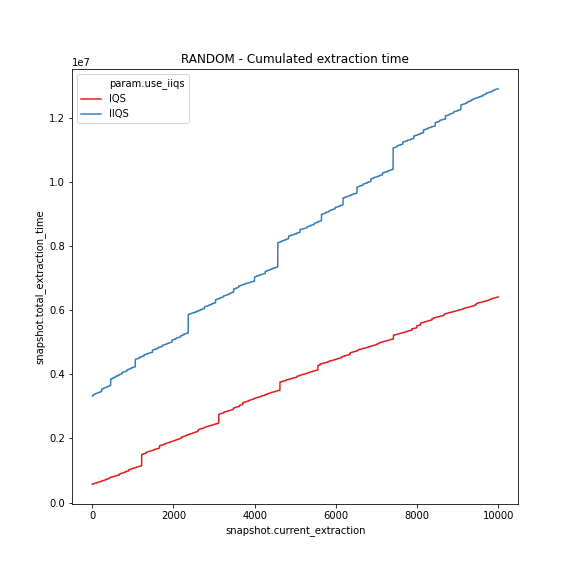
\includegraphics[width=0.40\textwidth]{./fragments/04_experimental_execution/images/01_basebenchmark_01_random_case.png.0_0.png}
        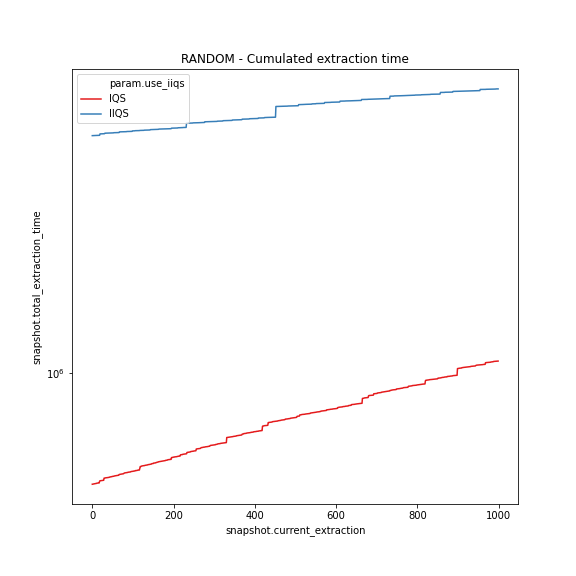
\includegraphics[width=0.40\textwidth]{./fragments/04_experimental_execution/images/01_basebenchmark_01_random_case.png.0_1.png}
        \caption{Cumulated extraction time}
        \label{FIG:BENCHMARK_01_RANDOM_CASE__0_0}
    \end{subfigure}

    \begin{subfigure}[b]{\textwidth}
        \centering
        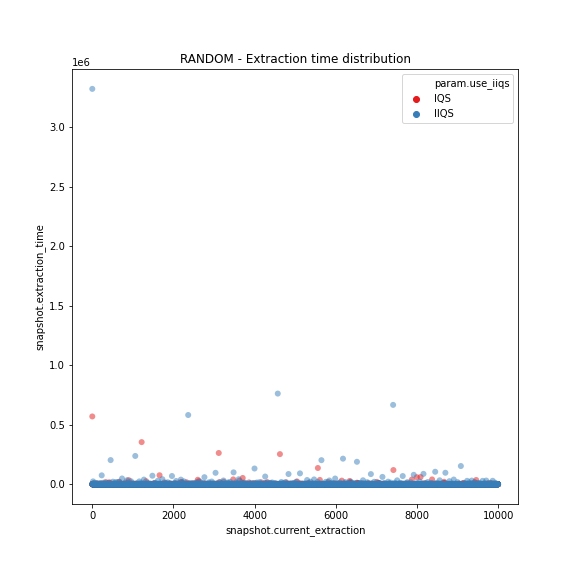
\includegraphics[width=0.40\textwidth]{./fragments/04_experimental_execution/images/01_basebenchmark_01_random_case.png.1_0.png}
        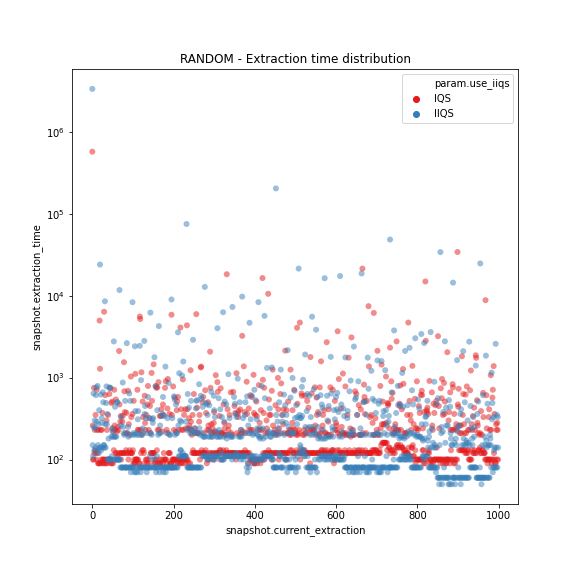
\includegraphics[width=0.40\textwidth]{./fragments/04_experimental_execution/images/01_basebenchmark_01_random_case.png.1_1.png}
        \caption{Extraction time}
        \label{FIG:BENCHMARK_01_RANDOM_CASE__0_0}
    \end{subfigure}

    \begin{subfigure}[b]{\textwidth}
        \centering
        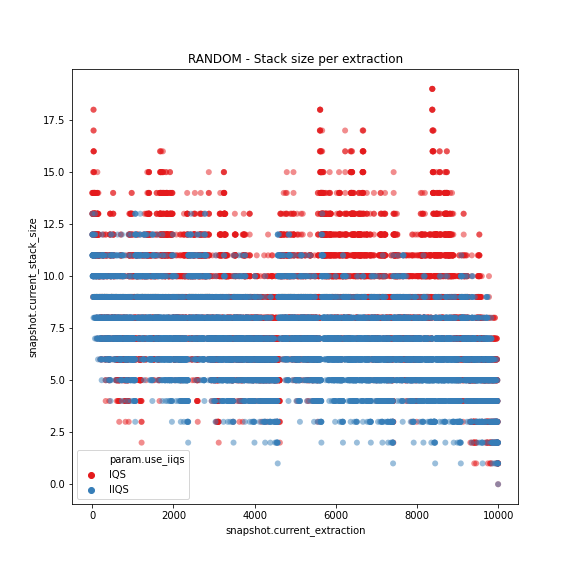
\includegraphics[width=0.40\textwidth]{./fragments/04_experimental_execution/images/01_basebenchmark_01_random_case.png.2_0.png}
        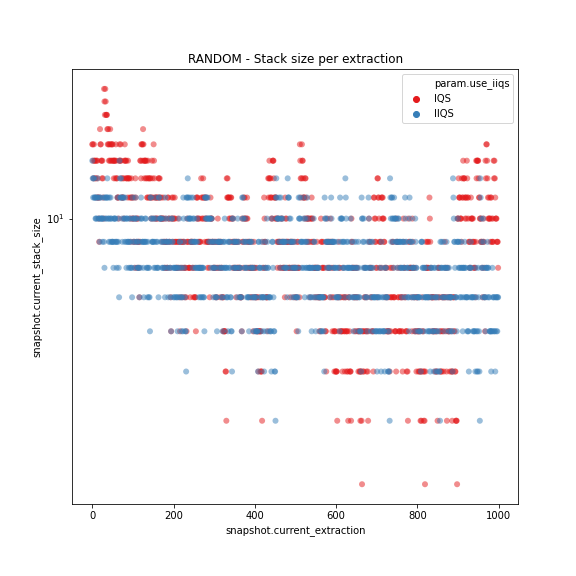
\includegraphics[width=0.40\textwidth]{./fragments/04_experimental_execution/images/01_basebenchmark_01_random_case.png.2_1.png}
        \caption{Stack size}
        \label{FIG:BENCHMARK_01_RANDOM_CASE__0_0}
    \end{subfigure}
    
    \caption{Base IQS and IIQS benchmark for a random sequence with $1\times10^5$ elements.}
       \label{FIG:BENCHMARK_01_RANDOM_CASE}
\end{figure}

As depicted in Figure \ref{FIG:BENCHMARK_01_RANDOM_CASE}, IIQS only shows a constant time added to IQS execution when solving a randomly ordered sequence. Despite forcing the pivot selection to the first element in the sequence, given that the sequence is randomly sorted, the first element on the sequence is randomly selected at all times. Random sequences transitively imply a random pivot selection case.\\

Another interesting aspect of both algorithms is that the stack size remains stable among all performed extractions. This is proof that in average, the stack does not grow asymptotically than $log_2(n)$.\\

\begin{figure}
    \centering
    \begin{subfigure}[b]{\textwidth}
        \centering
        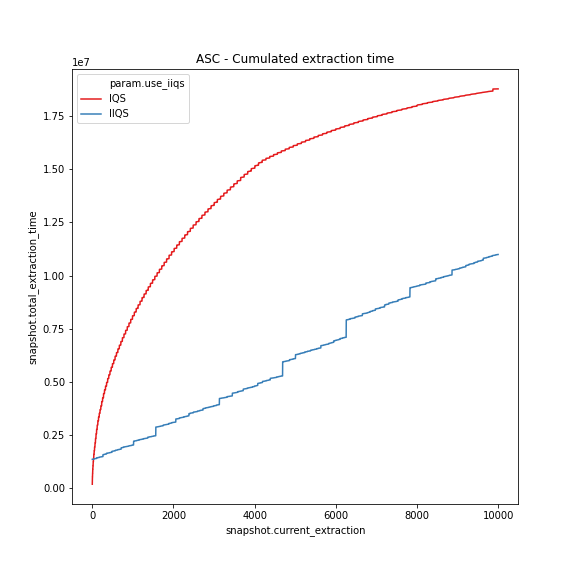
\includegraphics[width=0.40\textwidth]{./fragments/04_experimental_execution/images/01_basebenchmark_02_sort_a_case.png.0_0.png}
        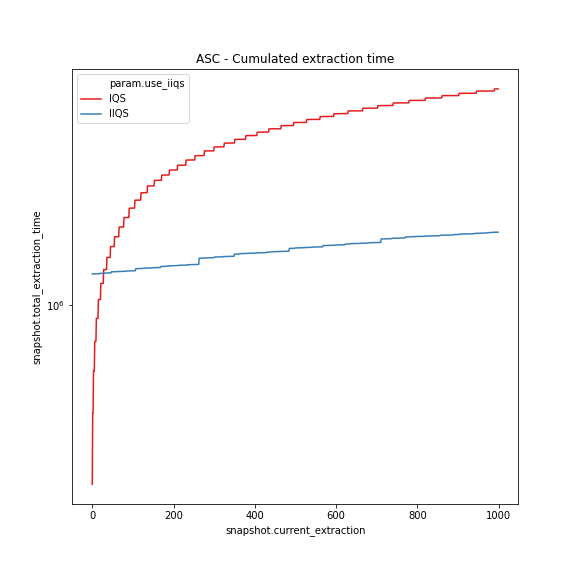
\includegraphics[width=0.40\textwidth]{./fragments/04_experimental_execution/images/01_basebenchmark_02_sort_a_case.png.0_1.png}
        \caption{Cumulated extraction time}
        \label{FIG:BENCHMARK_02_ASC_CASE__0_0}
    \end{subfigure}

    \begin{subfigure}[b]{\textwidth}
        \centering
        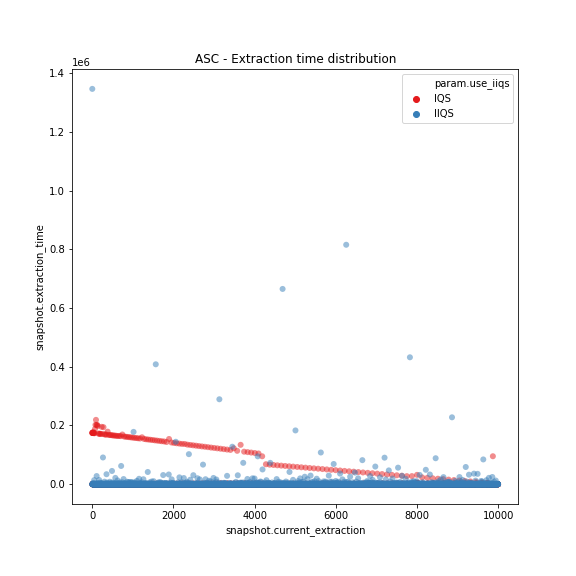
\includegraphics[width=0.40\textwidth]{./fragments/04_experimental_execution/images/01_basebenchmark_02_sort_a_case.png.1_0.png}
        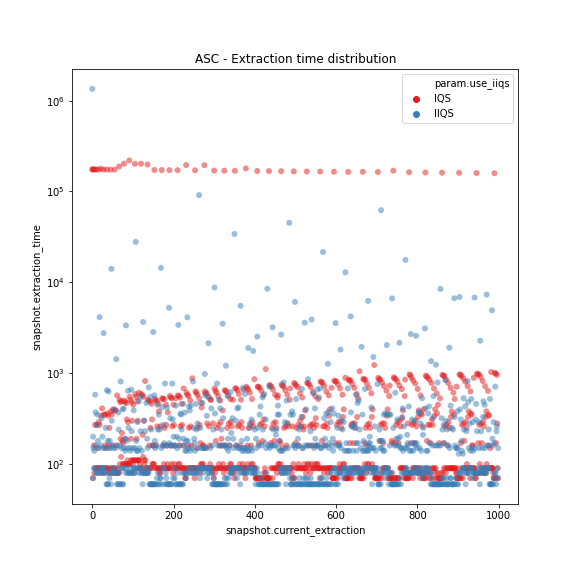
\includegraphics[width=0.40\textwidth]{./fragments/04_experimental_execution/images/01_basebenchmark_02_sort_a_case.png.1_1.png}
        \caption{Extraction time}
        \label{FIG:BENCHMARK_02_ASC_CASE__0_0}
    \end{subfigure}

    \begin{subfigure}[b]{\textwidth}
        \centering
        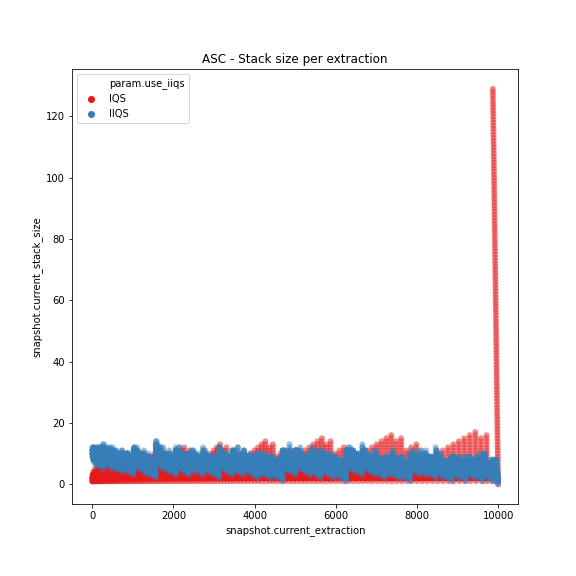
\includegraphics[width=0.40\textwidth]{./fragments/04_experimental_execution/images/01_basebenchmark_02_sort_a_case.png.2_0.png}
        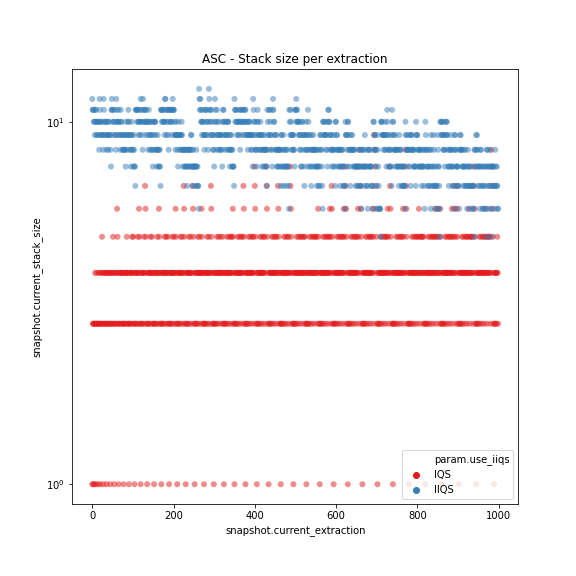
\includegraphics[width=0.40\textwidth]{./fragments/04_experimental_execution/images/01_basebenchmark_02_sort_a_case.png.2_1.png}
        \caption{Stack size}
        \label{FIG:BENCHMARK_02_ASC_CASE__0_0}
    \end{subfigure}
    
    \caption{Base IQS and IIQS benchmark for a ascending sequence with $1\times10^5$ elements.}
    \label{FIG:BENCHMARK_02_ASC_CASE}
\end{figure}

When fixing the pivot selection to the first element in the sequence, we are forcing a synthetic best case for the first extraction performed on IQS, as it is only required to run a partition which yields the element on the same position as it is being found. it is shown on Figure \ref{FIG:BENCHMARK_02_ASC_CASE}. 

There is one noticeable difference between this experiment and the original study and is that the stack in our case grows, but barely reaching the minimum expected on the average case. This is caused by the implementation of the partition algorithm. Usually a partition algorithm uses two pivots which converge to the index of the expected pivot position, but for a repeated case scenario such implementation is not feasible, as when repeated elements are found such indices need to move segments of the sequence when displaced, and there is no guarantee on the repeated property the next element in the iteration.\\

The purpose of this work is to study the behaviour of our algorithms in scenarios which has a closer match to reality and under the same conditions. For such effects, a Dutch-Flag problem implementation is used as our partition algorithm. The implementation details of this algorithm can be found on Section \ref{SUBSEC:DUTCH_FLAG_PROBLEM}.\\

On this implementation, since the partitioning swaps an element to the back of the to-be-partitioned segment, on the last step the last element alternates positions with the first on the partitioned sequence, as such, when the next element in the left-most position is selected, it ends being an element which belongs to the end of the array, instead of being the first on all cases.\\

Even on this scenario, there the stack size does not grow larger than the minimum expected size for a random case, which is an inefficient usage of the stack, causing the degradation of the algorithm. Even if some pivots are stored on them, as such pivots do not contribute to reduce the search space, there is no reduction on the execution time for subsequent calls.\\

\begin{figure}
    \centering
    \begin{subfigure}[b]{\textwidth}
        \centering
        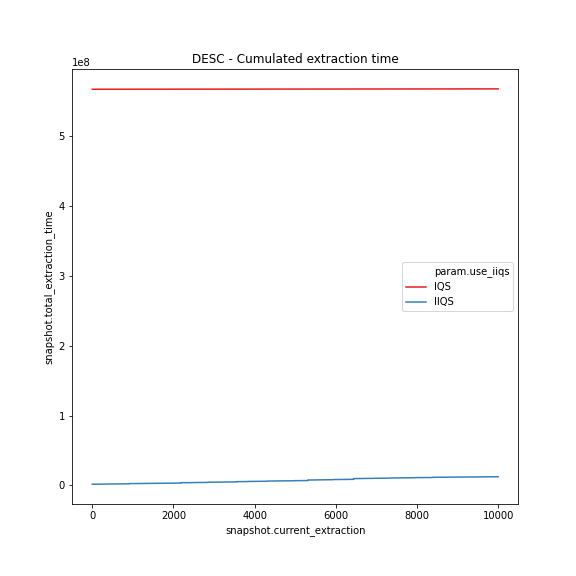
\includegraphics[width=0.40\textwidth]{./fragments/04_experimental_execution/images/01_basebenchmark_03_sort_d_case.png.0_0.png}
        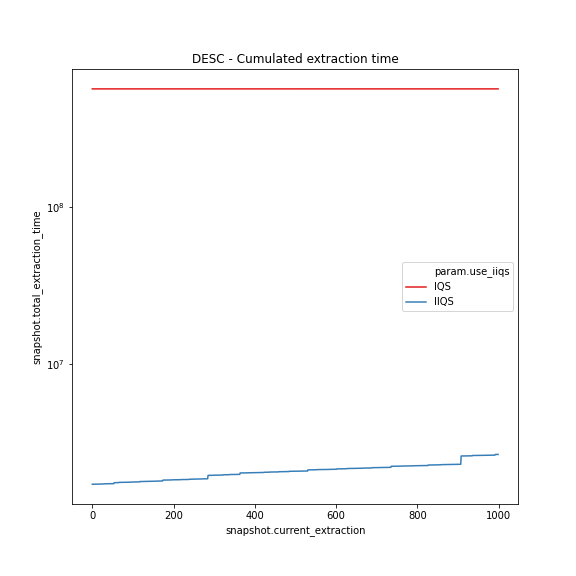
\includegraphics[width=0.40\textwidth]{./fragments/04_experimental_execution/images/01_basebenchmark_03_sort_d_case.png.0_1.png}
        \caption{Cumulated extraction time}
        \label{FIG:BENCHMARK_03_DESC_CASE__0_0}
    \end{subfigure}

    \begin{subfigure}[b]{\textwidth}
        \centering
        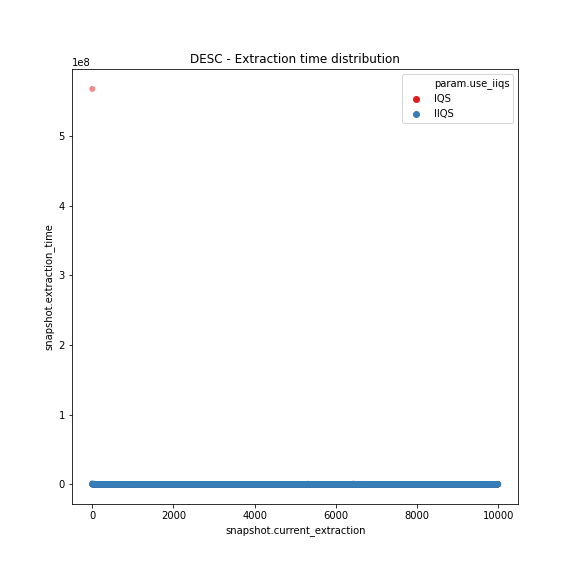
\includegraphics[width=0.40\textwidth]{./fragments/04_experimental_execution/images/01_basebenchmark_03_sort_d_case.png.1_0.png}
        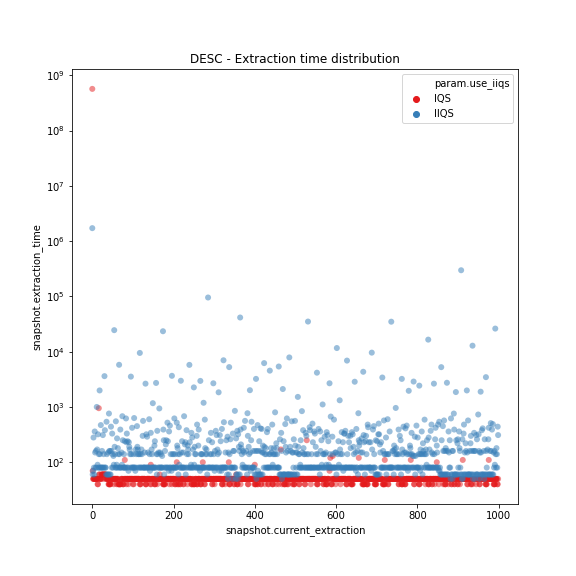
\includegraphics[width=0.40\textwidth]{./fragments/04_experimental_execution/images/01_basebenchmark_03_sort_d_case.png.1_1.png}
        \caption{Extraction time}
        \label{FIG:BENCHMARK_03_DESC_CASE__0_0}
    \end{subfigure}

    \begin{subfigure}[b]{\textwidth}
        \centering
        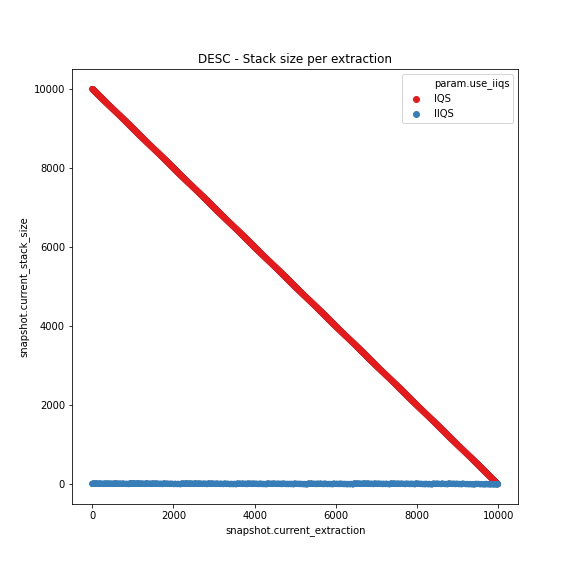
\includegraphics[width=0.40\textwidth]{./fragments/04_experimental_execution/images/01_basebenchmark_03_sort_d_case.png.2_0.png}
        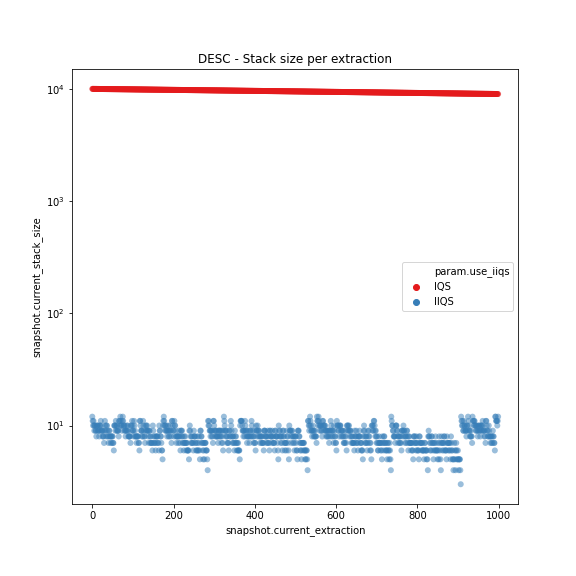
\includegraphics[width=0.40\textwidth]{./fragments/04_experimental_execution/images/01_basebenchmark_03_sort_d_case.png.2_1.png}
        \caption{Stack size}
        \label{FIG:BENCHMARK_03_DESC_CASE__0_0}
    \end{subfigure}
    
    \caption{Base IQS and IIQS benchmark for a descending sequence with $1\times10^5$ elements.}
    \label{FIG:BENCHMARK_03_DESC_CASE}
\end{figure}

The most extreme case for IQS is when the pivot selection always yields an element which does not reduce the search space --not for a useful value at least-- and the stack gets populated with all the elements at the first call as it can be seen on Figure \ref{FIG:BENCHMARK_03_DESC_CASE}. We can achieve this case by forcing the pivot selection to the first element on a decreasing sorted sequence. Then all the extractions yield the last element in the sequence, causing it to be stored on the stack and reducing the next iteration length by just one element without swapping any element on it.\\

As it can be seen, for the both three cases that can be found --synthetically-- on IQS, its introspective version performs with the same behaviour on all of them, but it does cost a fixed constant time more than the original version. In this context it is useful to remember that the purpose of incremental sorting algorithms is to speed up the first calls under the premise that the number of minima extracted is unknown while preserving the optimal asymptotic complexity in case of sorting the entire sequence. In this regard, IIQS manages to perform just as expected.\\

\subsection{Influence of repeated elements}

The question at hand now is what happens when repeated elements are found on the sequence. As mentioned before, this is the reason behind the change of the partition algorithm. In contrast to the original study, now we need to introduce three new factors to considerate:

\begin{itemize}
    \item \textbf{Number of classes}: How many classes have the repeated portion of the sequence.
    \item \textbf{Amount of random noise}: How many unique elements are present on the sequence.
    \item \textbf{Redundant bias}: Bias of the partition algorithm to deliver the pivot in regard of the repeated sequence.
\end{itemize}

Whilst not notorious, we from now on consider any distribution of the repeated element classes a instance of a uniformly distributed sequence. We can make this assumption based on how IQS works, as it reduces in average case by half on each iteration. Thus, for any distribution, the complexity toll is paid by the largest class found on the sequence.\\

\begin{figure}
    %BENCHMARK_05_CLASSES
    %01_basebenchmark_05_classes
    \centering
    \begin{subfigure}[b]{\textwidth}
        \centering
        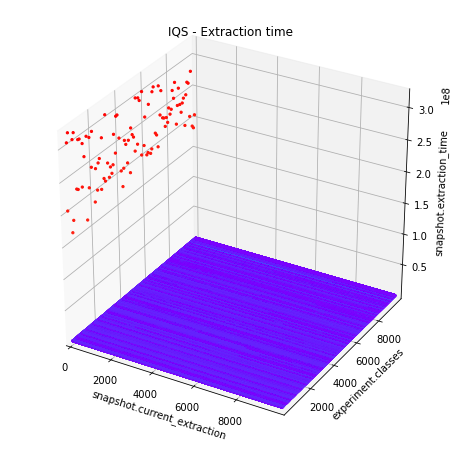
\includegraphics[width=0.40\textwidth]{./fragments/04_experimental_execution/images/01_basebenchmark_05_classes.png.1_0.png}
        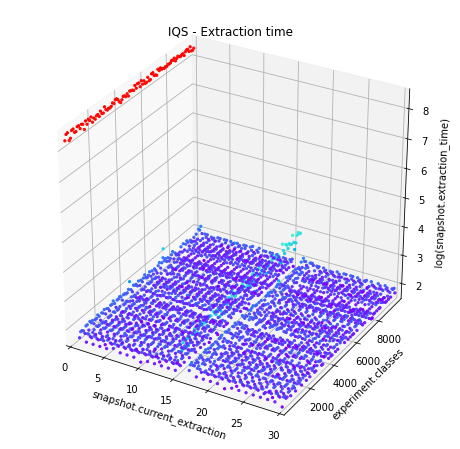
\includegraphics[width=0.40\textwidth]{./fragments/04_experimental_execution/images/01_basebenchmark_05_classes.png.1_1.png}
        \caption{IQS}
        \label{FIG:BENCHMARK_05_CLASSES__0_0}
    \end{subfigure}

    \begin{subfigure}[b]{\textwidth}
        \centering
        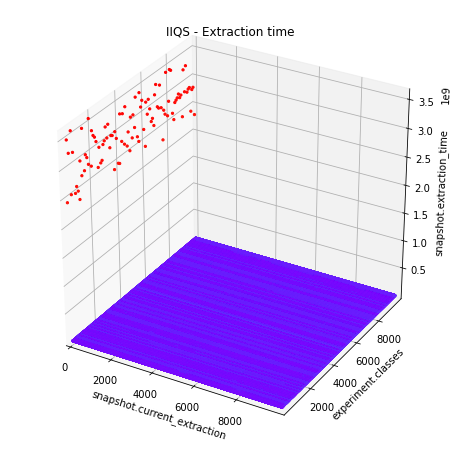
\includegraphics[width=0.40\textwidth]{./fragments/04_experimental_execution/images/01_basebenchmark_05_classes.png.0_1.png}
        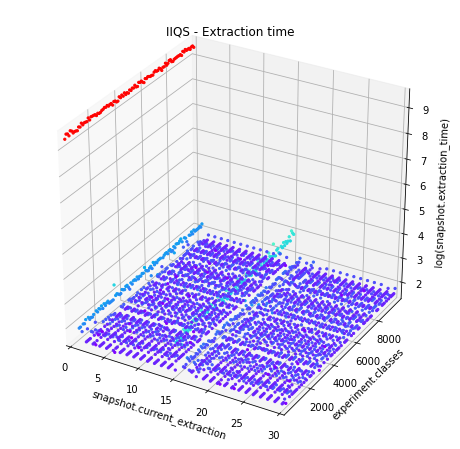
\includegraphics[width=0.40\textwidth]{./fragments/04_experimental_execution/images/01_basebenchmark_05_classes.png.0_2.png}
        \caption{IIQS}
        \label{FIG:BENCHMARK_05_CLASSES__0_1}
    \end{subfigure}

    \caption{Base IQS and IIQS benchmark for class impact on extraction time.}
    \label{FIG:BENCHMARK_05_CLASSES}
\end{figure}

\begin{figure}
    %BENCHMARK_05_CLASSES
    %01_basebenchmark_08_extraction_bias
    \centering
    \begin{subfigure}[b]{0.45\textwidth}
        \centering
        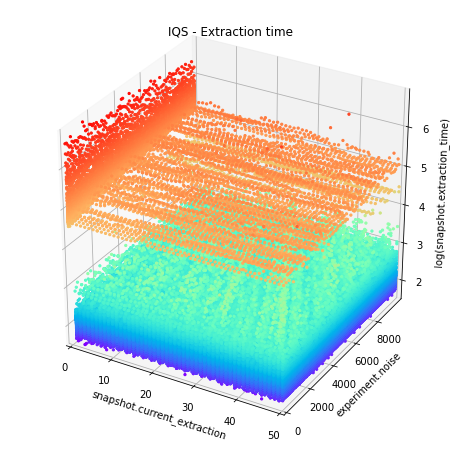
\includegraphics[width=0.9\textwidth]{./fragments/04_experimental_execution/images/01_basebenchmark_08_extraction_bias.png.1_0.png}
        % 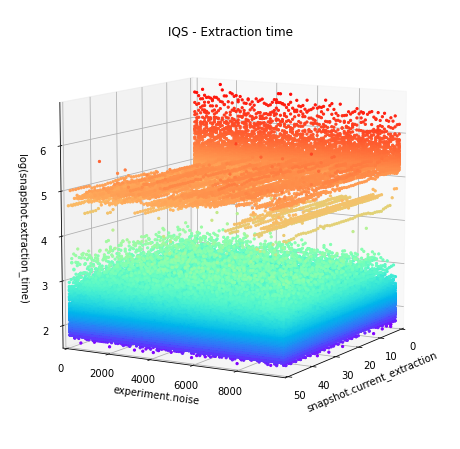
\includegraphics[width=0.40\textwidth]{./fragments/04_experimental_execution/images/01_basebenchmark_08_extraction_bias.png.1_1.png}
        \caption{IQS}
        \label{FIG:BENCHMARK_05_CLASSES__0_0}
    \end{subfigure}
    \hfill
    \begin{subfigure}[b]{0.45\textwidth}
        \centering
        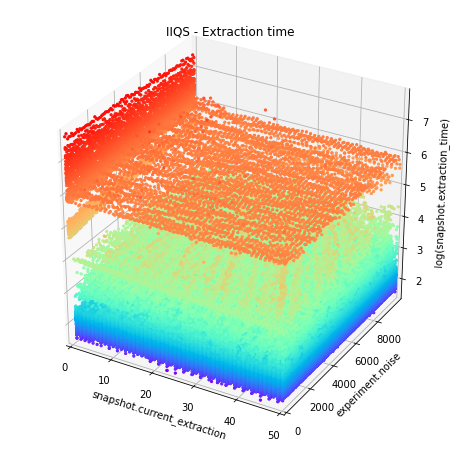
\includegraphics[width=0.9\textwidth]{./fragments/04_experimental_execution/images/01_basebenchmark_08_extraction_bias.png.0_0.png}
        %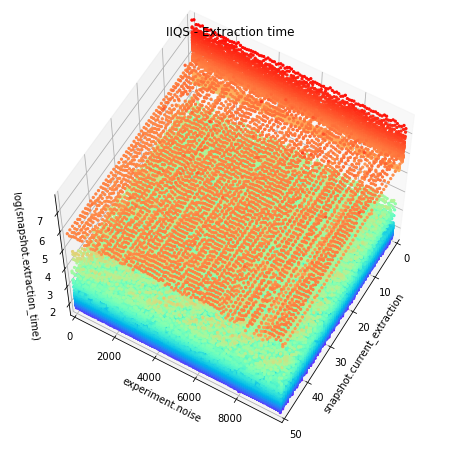
\includegraphics[width=0.40\textwidth]{./fragments/04_experimental_execution/images/01_basebenchmark_08_extraction_bias.png.0_1.png}
        \caption{IIQS}
        \label{FIG:BENCHMARK_05_CLASSES__0_1}
    \end{subfigure}

    \caption{Base IQS and IIQS benchmark for random noise impact on extraction time.}
    \label{FIG:BENCHMARK_05_CLASSES}
\end{figure}

As for the random noise in the sequence\footnote{We define as the random noise as the number of elements which does not belong to any controlled classes for the experiment. In this case, how many random elements are introduced as fillers on the array.}, as by itself as it does not make any visible changes on the behaviour of the algorithm in relation to its iterations. This is important, because the fact that a single class with low noise represents a case with the same behaviour as found on the worst case of IQS for both algorithms, as it can be checked on Figure~\ref{FIG:BENCHMARK_04_SINGLE_CLASS}.\\


\begin{figure}
    %BENCHMARK_04_SINGLE_CLASS
    %01_basebenchmark_04_single_class
    \centering
    \begin{subfigure}[b]{\textwidth}
        \centering
        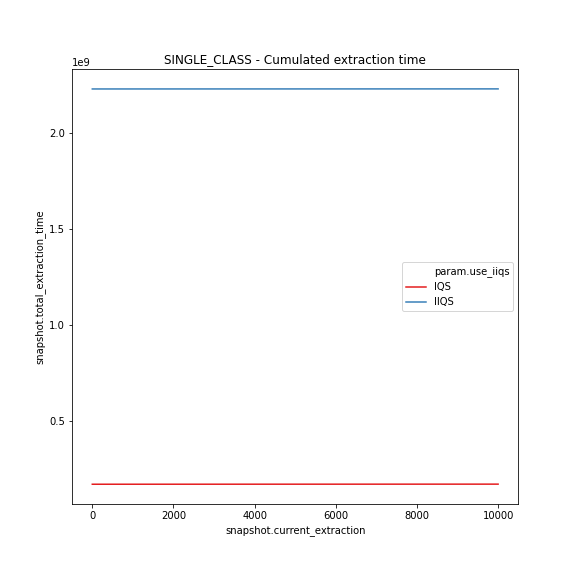
\includegraphics[width=0.40\textwidth]{./fragments/04_experimental_execution/images/01_basebenchmark_04_single_class.png.0_0.png}
        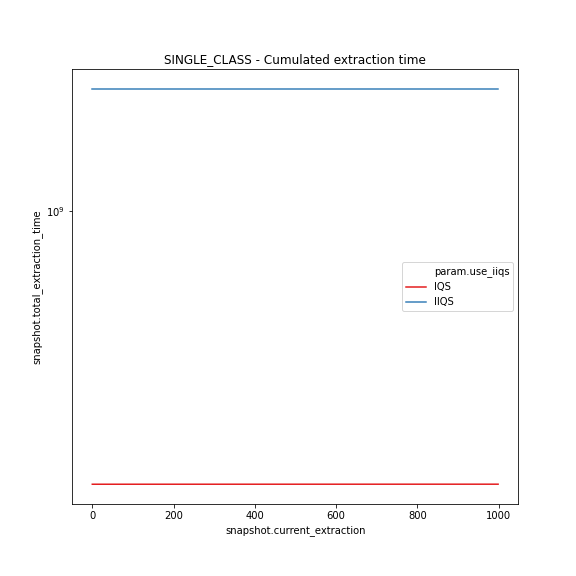
\includegraphics[width=0.40\textwidth]{./fragments/04_experimental_execution/images/01_basebenchmark_04_single_class.png.0_1.png}
        \caption{Cumulated extraction time}
        \label{FIG:BENCHMARK_04_SINGLE_CLASS__0_0}
    \end{subfigure}

    \begin{subfigure}[b]{\textwidth}
        \centering
        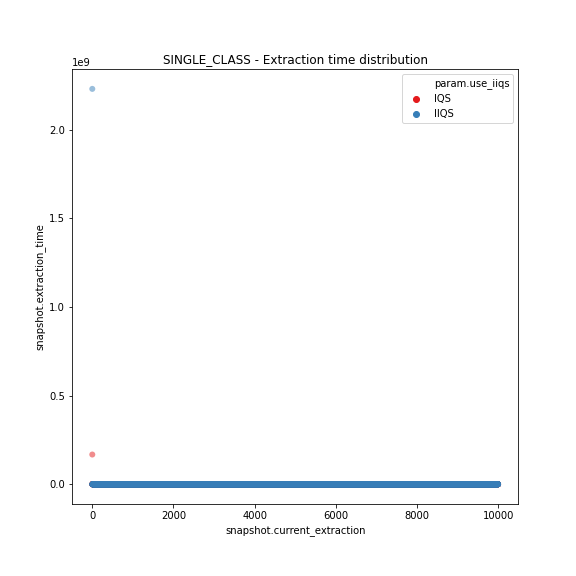
\includegraphics[width=0.40\textwidth]{./fragments/04_experimental_execution/images/01_basebenchmark_04_single_class.png.1_0.png}
        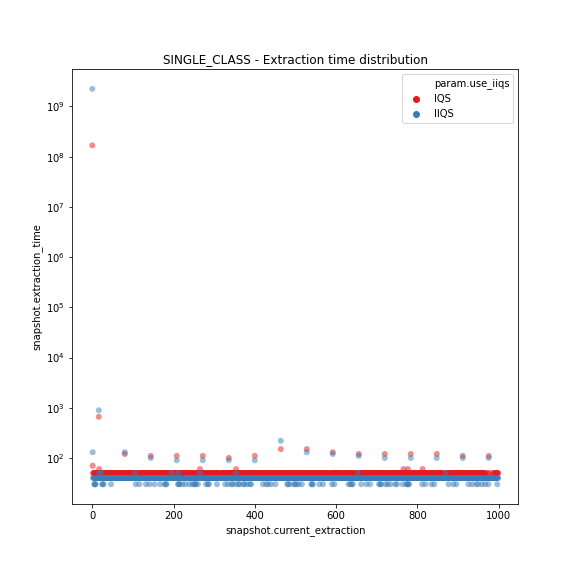
\includegraphics[width=0.40\textwidth]{./fragments/04_experimental_execution/images/01_basebenchmark_04_single_class.png.1_1.png}
        \caption{Extraction time}
        \label{FIG:BENCHMARK_04_SINGLE_CLASS__0_0}
    \end{subfigure}

    \begin{subfigure}[b]{\textwidth}
        \centering
        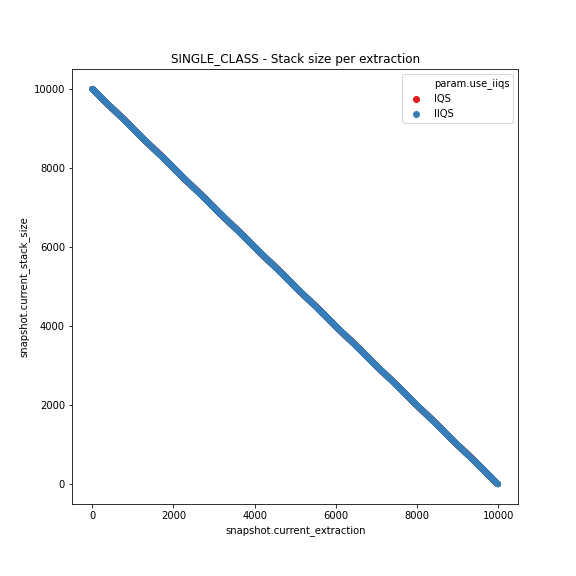
\includegraphics[width=0.40\textwidth]{./fragments/04_experimental_execution/images/01_basebenchmark_04_single_class.png.2_0.png}
        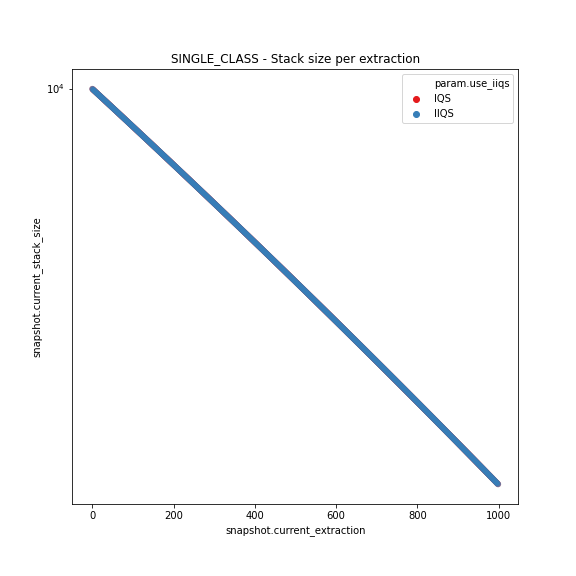
\includegraphics[width=0.40\textwidth]{./fragments/04_experimental_execution/images/01_basebenchmark_04_single_class.png.2_1.png}
        \caption{Stack size}
        \label{FIG:BENCHMARK_04_SINGLE_CLASS__0_0}
    \end{subfigure}
    
    \caption{Base IQS and IIQS benchmark for a random sorted sequence with $1\times10^5$ repeated elements.}
    \label{FIG:BENCHMARK_04_SINGLE_CLASS}
\end{figure}

At first glance there is no sign of the number of classes affecting the overall running time of the algorithm, as the Figure \ref{FIG:BENCHMARK_05_CLASSES} exhibits a similar behaviour to the one found on both IQS and IIQS, except for a small decrease of the extraction time when less classes are found. Thus we can conclude that the mere fact of having at least a single repeated element can make our algorithm to fall into a worst-case scenario, comparable to the same intended to avoid on the original IIQS implementation.\\

\FloatBarrier